\documentclass{paper}
\usepackage{geometry}
\usepackage{amsmath}
\usepackage{setspace}
\usepackage{natbib}
\usepackage{float}
\usepackage{graphicx}
\usepackage{url}
\usepackage{caption}
\let\oldref\ref
\renewcommand{\ref}[1]{(\oldref{#1})}
\def\bitcoin{%
  \leavevmode
  \vtop{\offinterlineskip %\bfseries
    \setbox0=\hbox{B}%
    \setbox2=\hbox to\wd0{\hfil\hskip-.03em
    \vrule height .3ex width .15ex\hskip .08em
    \vrule height .3ex width .15ex\hfil}
    \vbox{\copy2\box0}\box2}}

\geometry{
	left = 1in,
	right = 1in,
	top = 1in,
	bottom = 1in
}

\graphicspath{{Figures/}}
\begin{document}
\title{The Financial Risks of Bitcoin}
\author{Joshua L. Eubanks}
\maketitle
    \begin{doublespacing}

\section{Introduction}
Bitcoin\footnote{I shall follow the standard convention of writing a capital B for the institution, and lower case b or the symbol $\bitcoin$ for the actual currency.} has become a popular cryptocurrency. Over the span of eight years, the spot price has been as low as \$0.06/$\bitcoin$ reached its peak at almost \$19,000/$\bitcoin$ in December. Although bitcoin has achieved rapid growth, it has been accompanied by high volatility. As a result of bitcoin's high variance and increasing popularity, centralized exchanges, such as the Chicago Mercantile Exchange (CME) and the Chicago Board Options Exchange (CBOE), opened bitcoin futures markets on December 15, 2017 and December 11, 2017, respectively. In addition, the firm BitPay facilitates bitcoin transactions for small business. Businesses can keep the bitcoin, or convert it directly to cash at the spot price at the time of the transaction. Essentially, BitPay ameliorates exchange rate risk and default risk for the low price of one percent per transaction fee (major credit card companies charge between three and six percent). How does BitPay offer such low rates? Why do people use bitcoin instead of their domestic currency? Why does the process of mining bitcoin use as much electricity as the country of Ireland?\footnote{Forbes: Bitcoin Mining Uses as Much Power as Ireland. Here's Why That's Not A Problem by Christopher Helman} Understanding the Bitcoin institution may explain why people are willing to spend time, effort, and resources in this market.

Bitcoin is a decentralized ledger system that rewards individuals (miners) in bitcoin that verify transactions (update ledger) between individuals. When someone mines, his or her goal is to find a unique block ID that, when sent through a hash function, generates a fixed number of leading zeros. The mining process takes 10 minutes on average and increases in difficulty as the number of miners increase to maintain that average by increasing the number of leading zeros required from the hash function. The first block created required 8 leading zeros; as of June 23 it requires 18 leading zeros.\footnote{This was gathered from BlockExplorer, a site that keeps a record of all bitcoin transactions.} The bitcoin rewards also diminish by half for every 210,000 coins mined, so there is a fixed amount of 21 million at the end. This kind of market would be similar to the oil market, as prices of oil increase, more firms would be willing to drill in Canada to obtain oil which requires more resources and effort. Recently,  miners have been receiving transaction fees on top of the bitcoin reward, because the transaction ledger (block) is a fixed size and the demand for bitcoin has increased. As a result of increasing demand, users of bitcoin will also pay a fee to the miner in order to be put on the transaction blocks sooner. Carriers of bitcoin prefer to use bitcoin because there is no central authority and their purchases are essentially anonymous.

\cite{hayes2018} developed a model in an attempt to show that bitcoin is not a `sham' as stated by individuals such as Warren Buffett and Robert Shiller.\footnote{CNBC: Warren Buffett says bitcoin is `probably rat poison squared'}\footnote{NYT: What is Bitcoin Really Worth? Don't Even Ask} In \citeauthor{hayes2018} model, he fits bitcoin spot prices to the cost of the mining hardware and the electricity costs. It appears to have a strong linear relationship, but did not fit well during the bubble at the end of 2017.

\cite{ozvatic2015} investigated contango versus normal backwardation and additionally studied the convenience yield risk associated with holding bitcoin. This study was before the introduction of centralized future exchanges and thus, data gathered was from a decentralized exchange (Orderbook) for futures prices. His results suggest strong evidence for contango with a convenience yield of $-72.71$ percent, and this is easily observed in his data because the futures prices were everywhere above spot prices until the maturity dates. He calculated the convenience yield risk to be $-0.32$ percent using the methodology outlined by \cite{gibsschw1990}. \cite{haleetal2018} suggested that due to the introduction of centralized futures markets, that this allowed pessimists to enter the market and will bring the price down again.

I shall follow a similar process to \citeauthor{ozvatic2015} in the first two models on estimating whether the market is in contango or normal backwardation. In \citeauthor{ozvatic2015}'s case, he calculated the convenience yield by assuming that the risk free rate of return is the treasury bill yield. I avoid making that assumption for calculating whether or not the market is in contango or normal backwardation by instead looking at the EDFs of the difference between the convenience yield and the risk free rate of return. Since there are two centralized exchanges for bitcoin futures, I also compare the EDFs across the two exchanges to investigate if there are any differences across the two. In the second model, I follow the same structure as \citeauthor{ozvatic2015} to calculate the convenience yield risk, then make a comparison between his calculations and mine.

Finally, I investigate BitPay's one percent transaction fee. This seems rather small considering credit card companies charge higher rates and they are not exposed to exchange rate risk as is the case with BitPay. I look at the short run volatility of bitcoin spot prices using Brownian motion and compare that to the miner's transaction fees.

\section{Models}
\subsection{Measuring Contango Versus Normal Backwardation}
Contango occurs when the futures price is above the expected spot price or when the convenience yield is less than the risk free rate. Normal backwardation is when futures price is below the spot price, or the convenience yield is greater than the risk free rate.
To establish the existence of either two states, I assume a no-arbitrage environment such that the following equation holds:
$$F_{t,T} = S_{t}e^{(r_{T-t} + u - c_{T-t})(T-t)}$$
where $T$ is the maturity time period, $t$ is the current time period, $F$ is futures, $S$ is spot, $r$ is the risk free rate, $u$ is the carrying cost, $c$ is the convenience yield.

The assumption of no arbitrage is not unlike the assumption that a firm minimizes cost. If the left-hand side were to be less than the right-hand side, then one could profit by buying futures contracts and awaiting delivery. If the left-hand side were greater than the right-hand side, one can buy bitcoin at the spot price and sell futures contracts. Since bitcoin does not have storage costs, unlike oil or coal, I assume $u = 0$. Minor algebraic manipulation yields the following:
\begin{align}
c_{T-t} - r_{T-t} &= \frac{\log(S_{t})-\log(F_{t,T})}{T-t}\label{cont}
\end{align}

The right-hand side of Equation \ref{cont} can be easily calculated and we can find the EDFs of the right hand side for the CME and the CBOE and construct confidence bands around them using the Dvoretzky-Kiefer-Wolfowitz inequality. Also, one can implement a two-Sample Kolomgorov-Smirnov test to see whether the EDFs are significantly different. The rejection region is given by the following formula for $\alpha = 0.05$:
$$\sup\limits_{x}\left|F_{CME,n}(x)- F_{CBOE,m}(x)\right| > 1.36\sqrt{\frac{n+m}{nm}}$$
Finally, from the data generated, I shall perform a simple hypothesis test of the means and see if the means are significantly different from zero. If not, this would state that the difference between the convenience yield and the risk free rate is not different from zero, thereby not exhibiting neither contango or normal backwardation. For this model, all of the daily spot prices and the futures contracts are used and $(T-t)$ would be found by taking the maturity date of the contract and subtracting that from the current time period.
\subsection{Estimating the Convenience Yield Risk}
\citeauthor{ozvatic2015} followed the model developed by \cite{gibsschw1990} to estimate convenience-yield risk by using:
\begin{align*}
F_{t} &= s_{t}\cdot\exp\left(-\delta_{t}\left[\frac{1-\exp(-\kappa T_{t})}{\kappa}\right]+ A(T_{t})\right)\\
A(T_{t}) &= \left(r-\alpha + \frac{\lambda_{t}}{\kappa}+\frac{\sigma^{2}_{\delta}}{2\kappa^{2}} - \frac{\sigma_{s}\sigma_{\delta}\rho}{\kappa}\right)T_{t}+ \frac{\sigma^{2}_{\delta}[1-\exp(-2\kappa T_{t})]}{4\kappa^{3}}\\
& + \left(\alpha\kappa - \lambda_{t} + \sigma_{s}\sigma_{\delta}\rho - \frac{\sigma^{2}_{\delta}}{\kappa} \right)\frac{[1-\exp(-\kappa T_{t})]}{\kappa^{2}}\\
\end{align*}
where the variables are as represented in the table below.
\begin{center}
\begin{tabular}{ c| l }
 Variable & Definition \\\hline
 $\alpha$ & Long run mean convenience yield \\  
 $\delta$ & instantaneous convenience yield\\
 $F$ & Price of Futures contract\\
 $\kappa$ & Speed of mean reversion \\
 $\lambda$ & Market price of convenience yield risk\\
 $\mu$ & Mean daily spot return\\
 $r$ & Risk free rate of return \\
 $\rho$ & Correlation of the two residuals $\varepsilon_{s}$, $\varepsilon_{\delta}$ \\
 $s$ & Spot Price \\ 
 $\sigma_{\delta}$ & Volatility of daily convenience yields\\
 $\sigma_{s}$ & Volatility of daily spot returns \\
 $T$ & Maturity date \\ 
\end{tabular}
\end{center}
$\delta$ will be calculated by adding the treasury bill yield to both sides of Equation \ref{cont}. Variables $F,S,T,$ and $r$ will be determined by the data collected; $\varepsilon_{s}$ and $\sigma_{s}$ will be estimated by finding the standard deviation and residuals of an Ornstein-Ulenbeck process on spot prices:
\begin{align}
\log\left(\frac{s_{t}}{s_{t-1}}\right) = a + b\log\left(\frac{s_{t-1}}{s_{t-2}}\right) + \varepsilon_{s} \label{ornstein}
\end{align}
and the other variables needed are found by this regression equation:
\begin{align}
\delta_{t} - \delta_{t-1} = \kappa\alpha + \kappa\delta_{t-1}+\varepsilon_{\delta} \label{delta}
\end{align}
From these values, I can implement a simulation to find the distribution of $\lambda$. 
\begin{align}
\lambda_{t} = \left(\frac{[1-\exp(-\kappa T_{t})]}{\kappa^{2}}-\frac{T_{t}}{\kappa}\right)^{-1}&\Bigg(\log(s_{t})-\log(F_{t}) -\delta_{t}\left(\frac{1-\exp^(-\kappa T_{t})}{\kappa}\right)\nonumber\\
&+ \left(r-\alpha +\frac{\sigma^{2}_{\delta}}{2\kappa^{2}} - \frac{\sigma_{s}\sigma_{\delta}\rho}{\kappa}\right)T_{t}+ \frac{\sigma^{2}_{\delta}[1-\exp(-2\kappa T_{t}])}{4\kappa^{3}}+ \left(\alpha\kappa + \sigma_{s}\sigma_{\delta}\rho - \frac{\sigma^{2}_{\delta}}{\kappa} \right)\frac{[1-\exp(-\kappa T_{t})]}{\kappa^{2}}\Bigg)\label{lambda}
\end{align}
For calculating the convenience-yield risk, I shall use the June futures contract from the Chicago Mercantile Exchange and assume that the risk free rate is the 90-day U.S. Treasury bill yield to calculate the convenience yield.
\subsection{Measuring the Volatility of bitcoin}
For measuring the volatility, I employ the discrete time approximation to geometric Brownian motion, which is given by the following formula:
\begin{align}
\log\left(\frac{S_{t}}{S_{0}}\right) = \mu + U_{t}\label{brown}
\end{align}
where $U_{t}$ is a Gaussian random variable having mean zero and variance $\sigma$. Once I obtain the mean and standard deviation of the spot prices, I can then simulate out N time periods to observe the volatility that a firm such as BitPay would incur. Since I am interested in the liquidity of BitPay, I use spot prices collected on thirty-minute intervals over the span of two months.
\section{Data}
\subsection{Spot Prices and 90-Day Treasury Bill Yield}
All of the data collected were from the Bloomberg terminal. I collected the daily spot prices from December 11, 2017 to June 1, 2018 to be used.

\begin{table}[H]
\centering
\begin{tabular}{|c | c | c | c |}\hline
Min. & Max. & Mean & St. Dev. \\\hline
6604 & 18674 & 10272 & 2965.71\\\hline
\end{tabular}
\caption{Summary Statistics for Daily bitcoin Spot Prices.}\label{dspot}
\end{table}

Additionally, to measure the volatility of the spot price in the short run, I 
collected the 30 minute prices from April 1, 2018 at 14:30 to June 1, 2018 at 10:00.
\begin{table}[H]
\centering
\begin{tabular}{|c | c | c | c |}\hline
Min. & Max. & Mean & St. Dev. \\\hline
6516 & 9747 & 8176 & 88.24\\\hline
\end{tabular}
\caption{Summary Statistics for bitcoin spot prices on 30 minute intervals.}\label{30spot}
\end{table}
I assume that a reasonable estimate of the risk free rate is the yield of the 90-day Treasury bill. I need an estimate of the risk free rate to determine the convenience yield risk.
\begin{table}[H]
\centering
\begin{tabular}{|c | c | c | c |}\hline
Min. & Max. & Mean & St. Dev. \\\hline
1.252 & 1.905 & 1.632 & 0.207\\\hline
\end{tabular}
\caption{Summary Statistics for 90 day U.S. Treasury bill yield in percent.}\label{yield}
\end{table}
\subsection{Futures Contracts}
The futures contracts were collected on a daily basis for contracts that mature from January to September from both the Chicago Mercantile Exchange and the Chicago Board of Options Exchange. For both markets, the contracts began at varying times depending upon the maturity month of the contract. Within each section, I provide a table to help illustrate the summary statistics along with the lengths of the contracts for each exchange.\footnote{End dates with an asterisk denote the last day of data collection, the contracts extend past the date.} Their breakdown of the contract specifications and collection dates are below. 

\subsubsection{Chicago Mercantile Exchange}
The data was collected on the interval of the first day that the contracts were available through the CME (starting December 15, 2017) until June 1, 2018. The CME's contracts are for 5 bitcoin at the time of maturity. Their prices were determined using the standard method, unlike the CBOE, which uses a Gemini auction which is operated by the Winklevoss twins. The contracts mature on the last Friday of the contract month. 

\begin{table}[H]
\centering
\begin{tabular}{|c | c  c | c | c | c | c | c|}\hline
Contract& Start & End & No. Days & Min. & Max. & Mean & St. Dev. \\\hline
Jan & Dec 15 & Jan 26 & 29  & 10355 & 19500 & 14099 & 2553.18 \\
Feb & Dec 15 & Feb 23 & 49  & 7260  & 19600 & 12225 & 3163.39 \\
Mar & Dec 15 & Mar 29 & 73  & 7230  & 19700 & 11245 & 3055.78 \\
Apr & Jan 24 & Apr 27 & 67  & 6630  & 11780 & 8958  & 1358.88 \\
May & Feb 21 & May 25 & 67  & 6620  & 11675 & 8713  & 1152.92 \\
Jun & Dec 15 & Jun $1^{*}$  & 118 & 6630  & 19900 & 10133 & 2929.51 \\ 
Jul & Apr 27 & Jun $1^{*}$  & 26  & 7340  & 9720  & 8540  & 787.86  \\
Aug & May 24 & Jun $1^{*}$  & 6   & 7365  & 7630  & 7517  & 103.17  \\
Sep & Mar 27 & Jun $1^{*}$  & 48  & 6635  & 8210  & 9775  & 907.54  \\\hline
\end{tabular}
\caption{Summary Statistics for CME bitcoin futures contracts.}\label{CME}
\end{table}

\subsubsection{Chicago Board of Options Exchange}
The data was collected on the interval of the first day that the contracts were available through the CBOE (December 11, 2017) until June 22, 2018.
The contract matures on the Wednesday of the third week in the contract month and is for 1 bitcoin per contract. As stated in the previous section the transfer of contracts is through an auction by the Gemini auction house. I obtained the last price agreed upon by the buyer and seller for each day.
\begin{table}[H]
\centering
\begin{tabular}{|c | c  c | c | c | c | c | c|}\hline
Contract& Start & End & No. Days & Min. & Max. & Mean & St. Dev. \\\hline
Jan & Dec 11 & Jan 17 & 28  & 10710 & 19055 & 15399 & 2101.51 \\
Feb & Dec 11 & Feb 14 & 48  & 7055  & 19185 & 12887 & 3433.51 \\
Mar & Dec 15 & Mar 14 & 68  & 7230  & 19700 & 11245 & 3209.80 \\
Apr & Jan 22 & Apr 18 & 63  & 6605  & 11735 & 9026  & 1450.17 \\
May & Feb 1  & May 16 & 75  & 6610  & 11800 & 8856  & 1177.84 \\
Jun & Feb 20 & Jun 13 & 82  & 6276  & 11800 & 8560  & 1260.61 \\ 
Jul & Mar 19 & Jun $22^{*}$  & 70  & 6145 & 9755  & 7962  & 967.84  \\
Aug & Apr 23 & Jun $22^{*}$  & 45  & 6159 & 9935  & 8077  & 1080.39  \\
Sep & May 21 & Jun $22^{*}$  & 25  & 6145 & 8432  & 7196  & 632.25  \\\hline
\end{tabular}
\caption{Summary Statistics for CBOE bitcoin futures contracts.}\label{CBOE}
\end{table}


\section{Results}
\subsection{Contango Versus Normal Backwardation}
As it it shown in the figure below, it is not as clear of a distinction between the spot price and the futures price as in \citeauthor{ozvatic2015}'s paper which suggests further investigation of Equation \ref{cont}.
\begin{figure}[H]
\centering
\includegraphics[width=0.5\textwidth]{SpotvFut.pdf}
\caption{Spot prices plotted with June futures from CME}\label{spotfut}
\end{figure}

Below are the EDFs of Equation \ref{cont} broken down by month where the blue line represents the CBOE and the black line represents the CME. It appears that some EDFs are potentially different than others within the month, however, some differences can be explained because some of the samples are relatively small. For example, there are only 6 data points for the CME futures contract that expires August, thus the two-Sample Kolmogorov-Smirnov tests fail to reject the hypothesis that they are different.
\begin{figure}[H]
\centering
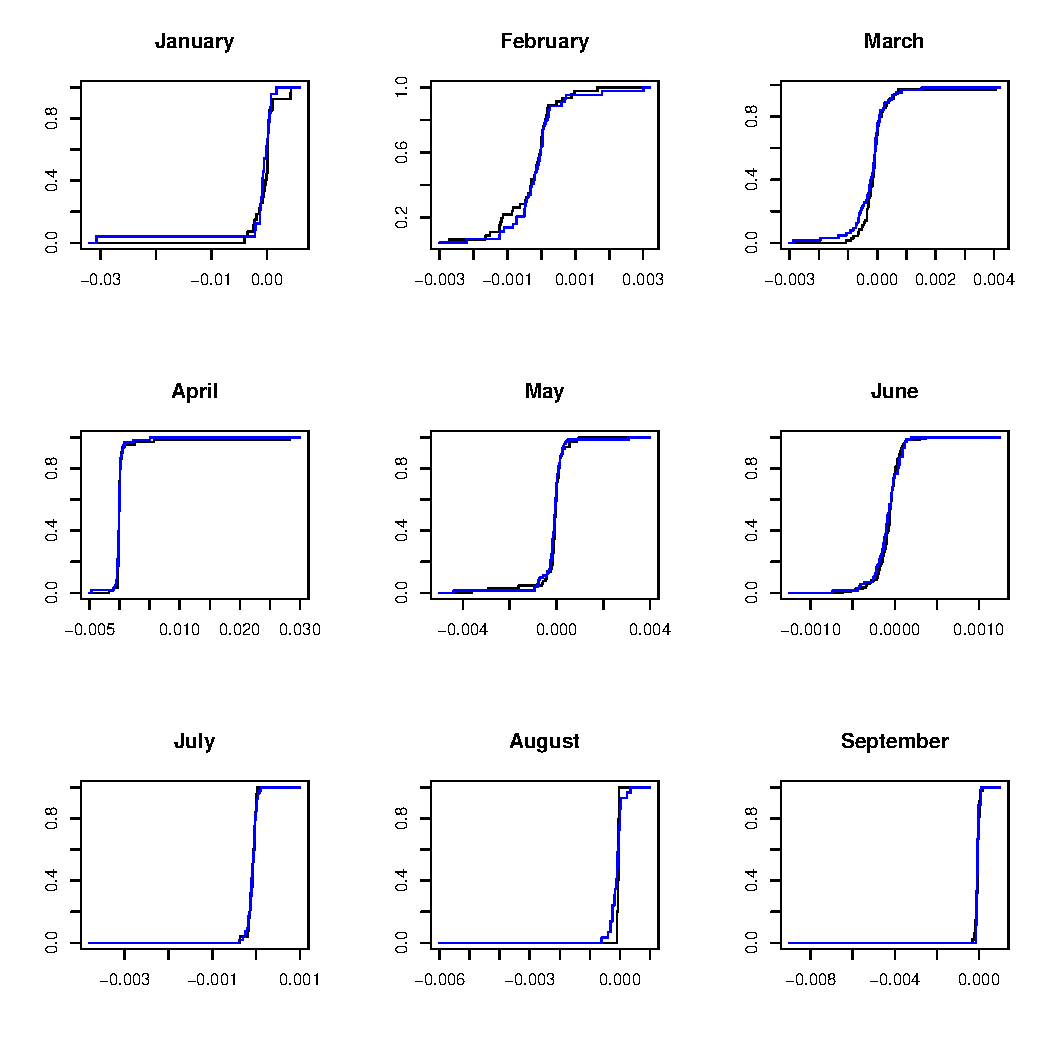
\includegraphics{CMEvsCBOEperMonth.pdf}
\caption{Comparison of EDFs by month}\label{comparison}
\end{figure}
Over the span of all futures contracts, we can observe the EDFs of the separate exchanges.
\begin{figure}[H]
\centering
\includegraphics[width=0.5\textwidth]{Overall.pdf}
\caption{Comparison of EDFs of Equation \ref{cont} for both exchanges}\label{overall}
\end{figure}
The two-Sample KS test did conclude that these distributions are statistically different since $0.093 > 0.091$. Additionally, I plotted the two EDFs with the 95 percent confidence interval using the DKW inequality.

\begin{figure}[H]
    \centering
    \begin{minipage}{0.5\textwidth}
        \centering
        \includegraphics[width=0.9\textwidth]{CME.pdf} % first figure itself
        \caption{EDF of Equation \ref{cont} for CME with 95\\ percent confidence interval}\label{edfcme}
    \end{minipage}\hfill
    \begin{minipage}{0.5\textwidth}
        \centering
        \includegraphics[width=0.9\textwidth]{CBOE.pdf} % second figure itself
        \caption{EDF of Equation \ref{cont} for CBOE with 95\\ percent confidence interval}\label{edfcboe}
    \end{minipage}
\end{figure}
Finally, a t-test was conducted on the $H_{0}: \mu = 0$ and $H_{A}: \mu \neq 0$ for both the CME and the CBOE.
\begin{table}[H]
\centering
\begin{tabular}{|c | c | c  c | c |}\hline
Exchange & Mean & Lower & Upper & pValue\\\hline
CME & $-0.00006$  & $-0.000215$ & 0.000095 & 0.4482\\
CBOE &$-0.000218$ & $-0.000392$ & $-0.000045$ & 0.01376\\\hline
\end{tabular}
\caption{T test and 95 percent confidence of Equation \ref{cont} for CME and CBOE}\label{tcont}
\end{table}
From Table \ref{tcont}, since the difference between the convenience yield and the risk free rate is negative, this suggests that the market is in contango for the CBOE. For the CME however, the market is neither in contango or normal backwardation.
\subsection{Convenience Yield Risk}
To obtain the variables needed to solve for $\lambda$, the convenience yield risk, I first estimated Equation \ref{ornstein} and obtained $\sigma^{2}_{s}$ = 0.00343 and $\varepsilon_{s}$ for the calculation of $\rho$. 

To ensure that this model is stationary, I plotted the auto correlation function and the partial auto correlation function of the residuals with a lag of 20 days. As you can see from Figures \ref{aSpot} and \ref{pSpot}, the residuals from the Ornstein-Ulenbeck process are not correlated.
\begin{figure}[H]
    \centering
    \begin{minipage}{0.5\textwidth}
        \centering
        \includegraphics[width=0.9\textwidth]{acfSpot.pdf} % first figure itself
        \caption{ACF of Equation \ref{ornstein} with 95 percent\\ confidence interval}\label{aSpot}
    \end{minipage}\hfill
    \begin{minipage}{0.5\textwidth}
        \centering
        \includegraphics[width=0.9\textwidth]{pacfSpot.pdf} % second figure itself
       \caption{PACF of Equation \ref{ornstein} with 95 percent\\ confidence interval}\label{pSpot}
    \end{minipage}
\end{figure}

From the estimation of Equation \ref{delta}, I obtained $\sigma_{\delta}$ = 0.0002124, $\varepsilon_{\delta}$ to calculate the correlation ($\rho = 0.2369015$), $\kappa = -0.0031982$, and $\kappa\alpha = 0.0001090$.

Once again, to ensure stationarity, I repeated the process before and found correlation between the residuals of this regression. This is an issue because this implies that the estimates of $\kappa\alpha$ and $\kappa$ are potentially biased and inconsistent.
\begin{figure}[H]
    \centering
    \begin{minipage}{0.5\textwidth}
        \centering
        \includegraphics[width=0.9\textwidth]{acfCon.pdf} % first figure itself
        \caption{ACF of Equation \ref{delta} with 95 percent\\ confidence interval}\label{aCon}
    \end{minipage}\hfill
    \begin{minipage}{0.5\textwidth}
        \centering
        \includegraphics[width=0.9\textwidth]{pacfCon.pdf} % second figure itself
        \caption{PACF of Equation \ref{delta} with 95 percent\\ confidence interval }\label{pCon}
    \end{minipage}
\end{figure}

From the previous values obtained from Equations \ref{ornstein} and \ref{delta} we can estimate $\lambda$ by simulating the coefficients from the previous results using Equation \ref{lambda} 2000 times. Below is the plot of the EDF and the histogram of $\lambda$.
\begin{figure}[H]
    \centering
    \begin{minipage}{0.5\textwidth}
        \centering
        \includegraphics[width=0.9\textwidth]{Lambda.pdf} % first figure itself
        \caption{EDF of Equation \ref{lambda}}\label{elam}
    \end{minipage}\hfill
    \begin{minipage}{0.5\textwidth}
        \centering
        \includegraphics[width=0.9\textwidth]{hist.pdf} % second figure itself
        \caption{Histogram of Equation \ref{lambda}}\label{lamhist}
    \end{minipage}
\end{figure}
A t-test was conducted and 95 percent confidence interval was constructed and is show below on Table \ref{tlam}.
\begin{table}[H]
\centering
\begin{tabular}{| c | c  c | c |}\hline
Mean & Lower & Upper & pValue\\\hline
0.005382773 & 0.005316357 & 0.005449188 & $<$ 2.2e$-16$\\\hline
\end{tabular}
\caption{T test and 95 percent confidence interval of $\lambda$}\label{tlam}
\end{table}
From this, we can conclude that $\lambda > 0$.
\subsection{Volatility of Spot Prices}
Plotted below is the spot price over the span of two months. As you can see, there are large changes over the last month with the largest drop of 10 percent within a 30 minute interval.
\begin{figure}[H]
    \centering
    \begin{minipage}{0.5\textwidth}
        \centering
        \includegraphics[width=0.9\textwidth]{30MinTrend.pdf} % first figure itself
        \caption{Logarithm of Spot Prices}\label{30trend}
    \end{minipage}\hfill
    \begin{minipage}{0.5\textwidth}
        \centering
        \includegraphics[width=0.9\textwidth]{PercentChange.pdf} % second figure itself
        \caption{Percent Change in Spot Prices}\label{perchan}
    \end{minipage}
\end{figure}
My initial thought as BitPay would want to remove the risk by instantly converting each transaction to USD. Since there are transaction fees by the miners, I wanted to make sure that the fees do not exceed 1 percent or else they would lose money on this policy. From \url{bitinfocharts.com/bitcoin/} I was able to collect the following information:
\begin{table}[H]
\centering
\begin{tabular}{| c | c  c | c |}\hline
 & Transaction Value (USD) & Fee & \% of Transaction\\\hline
Average & \$31,916 & \$0.889 & 0.002785437\\
Median & \$402.6 & \$0.166 & .04123199\\\hline
\end{tabular}
\caption{Transaction fees}\label{trans}
\end{table}
From this, I could say that this policy could be a potential safety net since as you can see below, the spot price can change as high as 4 percent and as low as 4 percent over 2 hours and over 20 percent increase, or more than a 30 percent decrease over one week. 
\begin{figure}[H]
    \centering
    \begin{minipage}{0.5\textwidth}
        \centering
        \includegraphics[width=0.9\textwidth]{2hrBrownian.pdf} % first figure itself
        \caption{Brownian Motion over two hours}\label{2Brown}
    \end{minipage}\hfill
    \begin{minipage}{0.5\textwidth}
        \centering
        \includegraphics[width=0.9\textwidth]{Brownian.pdf} % second figure itself
        \caption{Brownian Motion over one week}\label{weBrown}
    \end{minipage}
\end{figure}

\section{Conclusion}
In conclusion, I have found that the market for the CBOE is still in contango similar to Ozvatic's paper, but the difference between the convenience yield and the risk free rate is much smaller than in Ozvatic's case of finding the convenience yield to be $-72.71$ percent. Any reasonable risk free rate will not make the difference positive. Although the market is in contango for the CBOE, it is not the case that the CME is in either contango or normal backwardation. I find differing results from Ozvatic in which I obtain a positive convenience yield risk, whereas Ozvatic's paper was $-0.32$ percent. This estimate of $\lambda$ is potentially biased and inconsistent because the residuals of Equation \ref{delta} are serially correlated. Upon simulating the percentage changes in spot prices within a two hour interval and over the span of a week, it appears to be best practice for BitPay to convert their transactions they facilitate to USD instantly to avoid the high volatility of spot prices.

\end{doublespacing}
\newpage
% http://www.cmegroup.com/trading/equity-index/us-index/bitcoin_contract_specifications.html
% http://cfe.cboe.com/cfe-products/xbt-cboe-bitcoin-futures/contract-specifications
\bibliographystyle{chicago}

\bibliography{References}

\end{document}